% !TeX spellcheck = ru_RU-Russian
% !TeX encoding = UTF-8 

\documentclass[14pt,a4paper]{extarticle}

\usepackage[russian]{babel}
\usepackage[utf8]{inputenc}
\usepackage{setspace} 
\usepackage[a4paper,
		left=30mm,
		right=10mm,
		top=20mm,
		bottom=20mm]{geometry}
\usepackage{amsmath}
\usepackage{amssymb}
\usepackage{amsthm}
\usepackage{graphicx} 
\usepackage{cite}
\usepackage{subfigure}
\usepackage{subcaption}
\usepackage{kprj} 

\NIR

\title{Метод выбора функции Ляпунова в моделях с дробно-рациональными правыми частями}
\author{М.Д.~Кирдин}
\authorfull{Кирдин Матвей Дмитриевич}
\group{ФН12-81Б}
\faculty{Фундаментальные науки}
\chair{Математическое моделирование}
\chief{А.П.~Крищенко}
\workyear{2024}
\facultyshort{ФН}
\chairshort{ФН12}
\chairhead{А.П.~Крищенко}

\onehalfspacing

\begin{document}
	\maketitle
	
	\tableofcontents
	 
	\section{Постановка задачи}
	
	Рассмотрим следующую пятимерную систему с положительными параметрами:
	\begin{equation}
		\begin{cases}
			\begin{aligned}
				\dot{x}_1 &= r_1x_1\left(1-\dfrac{x_1}{c_1}\right)-\dfrac{1}{x_4+e_1}(\alpha_1x_2+\alpha_2x_3)\dfrac{x_1}{x_1+k_1},\\
				\dot{x}_2 &= r_2x_2\left(1-\dfrac{x_2}{c_2}\right)+\dfrac{x_5}{k_4+x_5}a_1\dfrac{1}{x_4+e_2}-\alpha_3\dfrac{x_1}{x_1+k_2}x_2,\\
				\dot{x}_3 &= a_2\dfrac{x_1}{k_5+x_4}-\mu_1x_3-\alpha_4\dfrac{x_1}{x_1+k_3}x_3,\\
				\dot{x}_4 &= s_1 + b_1x_1-\mu_2x_4,\\
				\dot{x}_5 &= b_2x_3-\mu_3x_5,
			\end{aligned}
		\end{cases}\label{eq:initial_system}
	\end{equation}
	где $x=(x_1, x_2, x_3, x_4, x_5)$ -- неотрицательные переменные, $t\ge0$ --- время.
	
	Введем следующие обозначения:
	\[\mathbb{R}^n_{+,0}=\left\{x=(x_1,\dots,x_n)\in\mathbb{R}^n:\, x_i\ge0,\, i=\overline{1,n}\right\},\,\mathbb{R}_{+,0}=\left\{x\in\mathbb{R}:\, x\ge0\right\}.\]
	
	Для данной системы найдем положения равновесия при помощи построения функций Ляпунова, а также условия их устойчивости, если таковые имеются. 
	
	\section{Основная часть}
	
	Рассмотрим следующий класс динамических систем:
	\[\dot{x}_i=f_i(x),\, x=(x_1,\dots,x_n)\in\mathbb{R}^{n}_{+,0},\, i=\overline{1,n},\]
	где правые части $f_i(x)$ --- некие дробно-рациональные функции (далее ДРФ) вида 
	\begin{equation*}
		g(x)=\dfrac{P(x)}{Q(x)},\quad l,\, m\in\mathbb{N}\cap\left\{0\right\}\}.
	\end{equation*}
	Здесь $P(x)$ и $Q(x)$ --- многочлены порядков $l$ и $m$ соответственно с отрицательными действительными корнями. 
	
	\begin{theorem}
		Для динамических систем данного  вида за функцию Ляпунова для внутреннего положения равновесия $x_0=(x_{1,0},\dots,x_{n,0})\in\mathbb{R}^n_{+}$ можно принять следующее выражение:
		\[V(x)=2\sum\limits_{i\in\sigma_1}\hat{k}_i(x_i-x_{i,0}-x_{i,0}\ln\dfrac{x_i}{x_{i,0}})+\dfrac{1}{2}\sum\limits_{j\in\sigma_2}\hat{k}_j(x_j-x_{j,0})^2,\]
		где $\sigma_1$ -- множество номеров функций $f_i(x)$ кратных $x_i$;\\ 
		$\sigma_2$ -- множество всех остальных номеров функций $f_j(x)$;\\
		$\hat{k}_i$ -- положительные параметры. 
		
		Производная такой функции в силу системы будет представима в виде квадратичной формы:
		\[\dot{V}(x)=(x-x_0)^{T}H(x)(x-x_0),\]
		где $H(x)$ -- симметричная функциональная матрица размера $n\times n$, координатными функциями которой являются константы либо рациональные функции. 
	\end{theorem}
	\begin{proof}
		Обозначим корни $Q_i(x)$ как $(-a_k)\in\mathbb{R}_{-},\, k=\overline{1,m}$, а корни $P_i(x)$ как $(-b_j)\in\mathbb{R}_{-},\, j=\overline{1,l}$. Тогда
		\begin{align*}
			Q_i(x)=&(x_{k_1}+a_1)\cdot\dots\cdot(x_{k_m}+a_m),\\
			P_i(x)=&(x_{j_1}+b_1)\cdot\dots\cdot(x_{j_l}+b_l).
		\end{align*}
		Здесь $j_1,\dots,j_l,k_1,\dots,k_m\in\left\{1,\dots,n\right\}$. Заметим, что во внутреннем ПР $x=x_0$ справедливо, что:
		\[f_i(x_0)=\dfrac{P_i(x_0)}{Q_i(x_0)}=0.\]
		
		На области $\mathbb{R}^n_{+}$ для $V(x)$ выполняются следующие условия:
		\[V(x)>0,\, V(x_0)=0,\, x_0\in D,\,x\in D\setminus\left\{x_0\right\}.\]
		Квадратичные слагаемые неотрицательно определены на области $\mathbb{R}^n_+$, слагаемые вида
		\[x_j-x_{j,0}-x_{j,0}\ln\dfrac{x_j}{x_{j,0}}\] 
		также неотрицательны в $\mathbb{R}^n_+$.
		Производная $V(x)$ в силу системы:
		\begin{multline*}
			\dot{V}(x)=\sum\limits_{i\in\sigma_1}\hat{k}_i\left(1-\dfrac{x_{i,0}}{x_i}\right)x_i\tilde{f}_i(x)+\sum\limits_{j\in\sigma_2}\hat{k}_j(x_j-x_{j,0})f_j(x)=\\
			=\sum\limits_{i\in\sigma_1}\hat{k}_i(x_i-x_{i,0})\tilde{f}_i(x)+\sum\limits_{j\in\sigma_2}\hat{k}_j(x_j-x_{j,0})f_j(x).
		\end{multline*}
		
		Воспользовавшись методом математической индукции покажем, что ДРФ $f_i(x)$ можно представить как набор произведений разностей $\Delta{}x_j$ и неких дробно-рациональных функций.
		
		При $l=0$ и $m=1$ имеем, что:
		\[f_i(x)=f_i(x)-f_i(x_0)=\dfrac{\Delta{}x_{k_1}}{(x_{k_1}+a_1)(x_{k_1,0}+a_1)}.\]
		
		При $l=0$ и $m=2$:
		\[f_i(x)=f_i(x)-f_i(x_0)=\dfrac{1}{(x_{k_1}+a_1)(x_{k_2}+a_2)}-\dfrac{1}{(x_{k_1,0}+a_1)(x_{k_2,0}+a_2)},\]
		\[f_i(x)=-\dfrac{\Delta{}x_{k_1}}{(x_{k_1}+a_1)(x_{k_1,0}+a_1)(x_{k_2,0}+a_2)}-\dfrac{\Delta{}x_{k_2}}{(x_{k_1}+a_1)(x_{k_2}+a_2)(x_{k_1,0}+a_1)},\]
		
		При $l=0$, $m\ge3$:
		\[f_i(x)=\dfrac{1}{(x_{k_1}+a_1)\cdot...\cdot(x_{k_m}+a_m)}-\dfrac{1}{(x_{k_1,0}+a_1)\cdot...\cdot(x_{k_m,0}+a_m)}.\]
		Тогда приведя дроби к общему знаменателю и совершив в числителе замену $x_{k_j}=\Delta x_{k_j} + x_{k_j,0}$ получим:
		\begin{multline*}
			f_i(x)=-\dfrac{\Delta x_{k_1}(x_{k_2,0}+a_1)\cdot...\cdot(x_{k_m,0}+a_m)}{(x_{k_1}+a_1)\cdot...\cdot(x_{k_m}+a_m)(x_{k_1,0}+a_1)\cdot...\cdot(x_{k_m,0}+a_m)}-\\
			-\dfrac{\Delta x_{k_1}\Delta x_{k_2}(x_{k_3,0}+a_1)\cdot...\cdot(x_{k_m,0}+a_m)}{(x_{k_1}+a_1)\cdot...\cdot(x_{k_m}+a_m)(x_{k_1,0}+a_1)\cdot...\cdot(x_{k_m,0}+a_m)}-...\\
			...-\dfrac{\Delta x_{k_1}\cdot...\cdot\Delta x_{k_{m-1}}(x_{k_m,0}+a_m)}{(x_{k_1}+a_1)\cdot...\cdot(x_{k_m}+a_m)(x_{k_1,0}+a_1)\cdot...\cdot(x_{k_m,0}+a_m)}-\\
			-\dfrac{\Delta x_{k_1}\cdot...\cdot\Delta x_{k_{m}}}{(x_{k_1}+a_1)\cdot...\cdot(x_{k_m}+a_m)(x_{k_1,0}+a_1)\cdot...\cdot(x_{k_m,0}+a_m)}.
		\end{multline*}
		Вынося поочередно множители $\Delta x_{k_j}$ из слагаемых, содержащих их, получим:
		\begin{multline*}
			f_i(x)=-\Delta x_{k_m}\dfrac{(x_{k_1,0}+a_1)\cdot...\cdot(x_{k_{m-1},0}+a_{m-1})}{(x_{k_1}+a_1)\cdot...\cdot(x_{k_m}+a_m)(x_{k_1,0}+a_1)\cdot...\cdot(x_{k_m,0}+a_m)}-\\
			-\Delta x_{k_{m-1}}\dfrac{(x_{k_1,0}+a_1)\cdot...\cdot(x_{k_{m-2},0}+a_{m-2})(\Delta x_{k_m}+x_{k_m,0}+a_m)}{(x_{k_1}+a_1)\cdot...\cdot(x_{k_m}+a_m)(x_{k_1,0}+a_1)\cdot...\cdot(x_{k_m,0}+a_m)}-...\\
			...-\Delta x_{k_1}\dfrac{\Delta x_{k_2}\cdot...\cdot\Delta x_{k_m}+...+(x_{k_2,0}+a_1)\cdot...\cdot(x_{k_m,0}+a_m)}{(x_{k_1}+a_1)\cdot...\cdot(x_{k_m}+a_m)(x_{k_1,0}+a_1)\cdot...\cdot(x_{k_m,0}+a_m)}.
		\end{multline*}
		Заметим, что каждое слагаемое начиная со третьего является произведением дроби 
		\[\dfrac{\Delta x_{k_j}}{(x_{k_j}+a_j)(x_{k_j,0}+a_j)}\] 
		и одного из предыдущих шагов индукции вплоть до шага $l=0,\, m=m-1$. Таким образом, 
		\begin{multline*}
			f_i(x)=-\dfrac{\Delta x_{k_m}}{(x_{k_1}+a_1)\cdot...\cdot(x_{k_m}+a_m)(x_{k_m,0}+a_m)}-...\\
			...-\dfrac{\Delta x_{k_1}}{(x_{k_1}+a_1)(x_{k_1,0}+a_1)\cdot...\cdot(x_{k_m,0}+a_m)}.
		\end{multline*}
		
		При $l=1$, $m\in\left\{2,\dots,n\right\}$:
		\[f_i(x)=\dfrac{(x_{j_1}+b_1)}{(x_{k_1}+a_1)\cdot...\cdot(x_{k_m}+a_m)}-\dfrac{(x_{j_1,0}+b_1)}{(x_{k_1,0}+a_1)\cdot...\cdot(x_{k_m,0}+a_m)}.\]
		Совершив в числителе первого слагаемого замену $x_{j_1}=\Delta x_{j_1} + x_{j_1,0}$ и раскрыв скобки можно получить следующую сумму:
		\begin{multline*}
			f_i(x)=\dfrac{\Delta x_{j_1}}{(x_{k_1}+a_1)\cdot...\cdot(x_{k_m}+a_m)}+\\
			+b_1\dfrac{(x_{k_1,0}+a_1)\cdot...\cdot(x_{k_m,0}+a_m)-(x_{k_1}+a_1)\cdot...\cdot(x_{k_m}+a_m)}{(x_{k_1}+a_1)\cdot...\cdot(x_{k_m}+a_m)(x_{k_1,0}+a_1)\cdot...\cdot(x_{k_m,0}+a_m)}.
		\end{multline*}
		Здесь второе слагаемое соответствует случаю, когда $l=0$ и $m\in\mathbb{N}\setminus\left\{1\right\}$, из чего предположение индукции работает также и в этом случае. 
		
		Рассмотрим случай, где $l > 1$ и $m\in\mathbb{N}\setminus\left\{1\right\}$.
		\[f_i(x)=\dfrac{(x_{j_1}+b_1)\cdot...\cdot(x_{j_l}+b_l)}{(x_{k_1}+a_1)\cdot...\cdot(x_{k_m}+a_m)}-\dfrac{(x_{j_1,0}+b_1)\cdot...\cdot(x_{j_l,0}+b_l)}{(x_{k_1,0}+a_1)\cdot...\cdot(x_{k_m,0}+a_m)}.\]
		Если разложить произвольное слагаемое в числителе первой дроби как $x_{j_p}=\Delta x_{j_p} + x_{j_p,0},\, p\in\left\{1,\dots,l\right\}$, то выражение преобразуется в сумму некой ДРФ и произведения разности $\Delta x_{j_p}$ и некоторой другой ДРФ. При этом заметим, что первое слагаемое будет соответствовать предыдущему шагу индукции, т.е. также может быть приведено к виду произведения разности и ДРФ.
		
		Таким образом, каждая функция $f_i(x)$ может быть представлена как
		\[f_i(x)=\sum\limits_{p\in\hat{\sigma}_i}(x_p-x_{p,0})\tilde{h}_p(x),\]    
		где $\tilde{h}_j(x)$ -- некие ДРФ или линейные функции, $\hat{\sigma}_i$ -- множество всех номеров $x_p,\, p\in\left\{1,\dots,n\right\}$, входящих в $f_i(x)$. Тогда производная $V(x)$ в силу системы примет вид:
		\[\dot{V}(x)=\sum\limits_{i\in\sigma_1}\hat{k}_i(x_i-x_{i,0})\sum\limits_{p\in\hat{\sigma}_i}(x_p-x_{p,0})\tilde{h}_{p}(x)+\sum\limits_{j\in\sigma_2}\hat{k}_j(x_j-x_{j,0})\sum\limits_{q\in\hat{\sigma}_j}(x_q-x_{q,0})\tilde{h}_{q}(x).\]
		Сложив все слагаемые с повторяющимися множителями $(x_i-x_{i,0})(x_j-x_{j,0})$ и положив равными нулю коэффициенты при множителях отсутствующих в сумме, получим квадратичную форму с симметричной функциональной матрицей $H$:
		\[\dot{V}(x)=(x-x_0)^{T}H(x-x_0).\qed\]
	\end{proof}
	
	\begin{theorem}
		Система \ref{eq:initial_system} имеет положения равновесия $P_1\left(0,\, 0,\,0,\,\dfrac{s_1}{\mu_2}\right)$ и $P_2\left(0,\, c_2,\,0,\,\dfrac{s_1}{\mu_2}\right)$ при положительных значениях параметров на границе множества $D$.  
	\end{theorem}
	
	\begin{theorem}
		Положение равновесия $P_1\left(0,0,0,\dfrac{s_1}{\mu_2},0\right)$ является неустойчивым в области $D$, а положение равновесия $P_2\left(0,c_2,0,\dfrac{s_1}{\mu_2},0\right)$ является асимптотически устойчивым в области $D$ при условии $k_1r_1s_1 + e_1k_1\mu_2r_1 < \alpha_1c_2\mu_2$ и неустойчивым в области $D$ при условии $k_1r_1s_1 + e_1k_1\mu_2r_1>\alpha_1c_2\mu_2$. При $k_1r_1s_1 + e_1k_1\mu_2r_1 = \alpha_1c_2\mu_2$ необходимо дополнительное исследование.
	\end{theorem}
	
	\begin{theorem}
		Положение $P_2\left(0,\, c_2,\,0,\,\dfrac{s_1}{\mu_2},\, 0\right)$ асимптотически устойчиво на инвариантной плоскости $G=\left\{x_1=x_3=x_5=0\right\}\cap D$. 
	\end{theorem}
	\begin{proof}
		На плоскости $G$ исходная система принимает следующий вид:
		\begin{equation}\label{eq:smol_sys}
			\begin{cases}
				\dot{x}_2=r_2x_2\left(1-\dfrac{x_2}{c_2}\right),\\
				\dot{x}_4=s_1-\mu_2x_4.
			\end{cases}
		\end{equation}
		Положение равновесия $P_2$ также будет являться положением равновесия для системы пониженного порядка \ref{eq:smol_sys} и эквивалентно точке $\tilde{P}_2\left(c_2,\, \dfrac{c_1}{\mu_2}\right)$ на плоскости $G$. Тогда рассмотрим следующую функцию Ляпунова:
		\[V(x_2,\, x_4)=2\hat{k}_1\left(x_2-c_2-c_2\ln\dfrac{x_2}{c_2}\right)+\dfrac{1}{2}\hat{k}_2\left(x_4-\dfrac{s_1}{\mu_2}\right)^2,\]
		где $\hat{k}_1,\hat{k}_2$ --- некоторые положительные числовые коэффициенты. Производная функции Ляпунова в силу системы таким образом:
		\[\dot{V}(x_2,\,x_4)=-(x_2-c_2)\hat{k}_1\dfrac{r_2}{c_2}(x_2-c_2)-\left(x_4-\dfrac{s_1}{\mu_2}\right)\mu_2\hat{k}_2\left(x_4-\dfrac{s_1}{\mu_2}\right).\]
		Ее можно представить как квадратичную форму следующего вида:
		\[\dot{V}(x_2,\, x_4)=\begin{pmatrix}
			x_2-c_2 & x_4-\dfrac{s_1}{\mu_2}
		\end{pmatrix}\begin{pmatrix}
			a_{11} & \dfrac{1}{2}a_{12}\\
			\dfrac{1}{2}a_{21} & a_{22}
		\end{pmatrix}\begin{pmatrix}
			x_2-c_2\\
			x_4-\dfrac{s_1}{\mu_2}
		\end{pmatrix},\]
		где $a_{11}=-\dfrac{r_2\hat{k}_1}{c_2},\, a_{12}=a_{21}=0,\, a_{22}=-\mu_2\hat{k}_2$. Пусть
		\[A=\begin{pmatrix}
			a_{11} & \dfrac{1}{2}a_{12}\\
			\dfrac{1}{2}a_{21} & a_{22}
		\end{pmatrix}=\begin{pmatrix}
		-\dfrac{r_2\hat{k}_1}{c_2} & 0\\
		0 & -\mu_2\hat{k}_2
		\end{pmatrix}\]
		Согласно критерию Сильвестра, если 
		\[a_{11}<0,\, \det A>0,\]
		то квадратичная форма, соответствующая $\dot{V}(x_2,\, x_4)$, отрицательно определена. Легко заметить, что 
		\begin{align*}
			a_{11} &= -\dfrac{r_2\hat{k}_1}{c_2}<0,\\
			\det A &= a_{11}a_{22}-\dfrac{1}{4}a^2_{12} = \dfrac{r_2\mu_2\hat{k}_1\hat{k}_2}{c_2}>0
		\end{align*}
		при положительных значениях параметров. Таким образом, 
		\[V(x)>0,\, \dot{V}(x)<0,\, x\in G\setminus\left\{\tilde{P}_2\right\},\]
		из чего $\tilde{P}_2$ асимптотически устойчиво на $G$.\qed
	\end{proof}
	
	\begin{theorem}
		Положение равновесия $P_1\left(0,0,0,\dfrac{s_1}{\mu_2},0\right)$ является неустойчивым на области $D$, а положение равновесия $P_2\left(0,c_2,0,\dfrac{s_1}{\mu_2},0\right)$ является асимптотически устойчивым в $D$ при условии $k_1r_1s_1 + e_1k_1\mu_2r_1< \alpha_1c_2\mu_2$ и неустойчивым при условии $k_1r_1s_1 + e_1k_1\mu_2r_1>\alpha_1c_2\mu_2$. При $k_1r_1s_1 + e_1k_1\mu_2r_1 = \alpha_1c_2\mu_2$ необходимо дополнительное исследование.
	\end{theorem}
	
	\begin{example}
		Рассмотрим систему \ref{eq:initial_system} при значениях параметров, данных в~\cite{model_params}. В \cite{model_params} указан только диапазон значений параметра $a_2$, поэтому положим, что $a_2=0.25$. Тогда имеет граничные положения равновесия
		\[P_1\left(0,\,0,\,0,\,9134.920635,\,0\right),\, P_2\left(0,\,1000000,\,0,\,9134.920635,\,0\right)\]
		и внутреннее положение равновесия
		\[P_3\left(875419.175014,\,943091.744167,\,151.680467,\,9135.646993,\,0.15168\right).\] 
		Проведем численное исследование полученной системы.
		
		Численно найдем матрицу Якоби системы с заданными параметрами в точке $P_1$: 
		\[\begin{pmatrix}
			0.010000& 0       & 0       & 0       & 0\\
			0       & 0.330700& 0       & 0       & 0\\
			0.000022& 0       &-0.007000& 0       & 0\\
			0       & 0       & 0       &-6.933988& 0\\
			0       & 0       &\phantom{-}0.000102& 0       &-0.102000
		\end{pmatrix}.\]
		Спектр данной матрицы имеет следующий вид:
		\begin{multline*}
			\lambda_1=-6.933988,\,\, \lambda_2=-0.102000,\\
			\lambda_3=-0.007000,\,\, \lambda_4=0.010000,\,\, \lambda_5=0.3307000.
		\end{multline*}
		Спектр содержит два положительных собственных значения, т.е. положение равновесия $P_1$ неустойчиво в $D$.
		
		Численно найдем матрицу Якоби системы с заданными параметрами  в точке $P_2$: 
		\[\begin{pmatrix}
			\phantom{-}0.007097& 0 &      0 &      0   &    0\\
			-0.718519&-0.293721& 0  &     0    &   0\\
			\phantom{-}0.000022& 0  &    -0.007000 &   0     &  0\\
			0     &  0   &     0    &    -6.933988&0\\
			0  &      0    &    \phantom{-}0.000102 & 0    &   -0.102000\\
		\end{pmatrix}.\]
		Спектр данной матрицы имеет следующий вид:
		\begin{multline*}
		\lambda_1=-6.933988,\,\, \lambda_2=-0.293721,\\
		\lambda_3=-0.102000,\,\, \lambda_4=-0.007000,\,\, \lambda_5=0.007097.
		\end{multline*}
		Собственное число $\lambda_5$ --- положительное действительное число, следовательно, положение равновесия $P_2$ неустойчиво в $D$.
		
		Матрица Якоби системы с заданными параметрами в точке $P_3$: 
		\[\begin{pmatrix}
			-0.009635&-0.000071&-0.000014& \phantom{-}0.003766&0\\
			-0.003638&-0.309228& 0       & 0.      & 0\\
  \phantom{-}0.000014& 0   &    -0.129571&-0.001766& 0\\
			 0       & 0     &   0     &  -6.933988& 0\\
			 0       & 0&\phantom{-}0.000102& 0   &   -0.102000 
		\end{pmatrix}.\]
		Спектр данной матрицы имеет следующий вид:
		\begin{multline*}
		\lambda_1=-6.933988,\,\, \lambda_2=-0.309229,\\
		 \lambda_3=-0.129571,\,\, \lambda_4=-0.102000,\,\, \lambda_5=-0.009634.
		\end{multline*}
		Все собственные значения являются отрицательными действительными числами, т.е. положение равновесия $P_3$ асимптотически устойчиво.
		
		\begin{figure}[h]
			\centering
			\subfigure[]{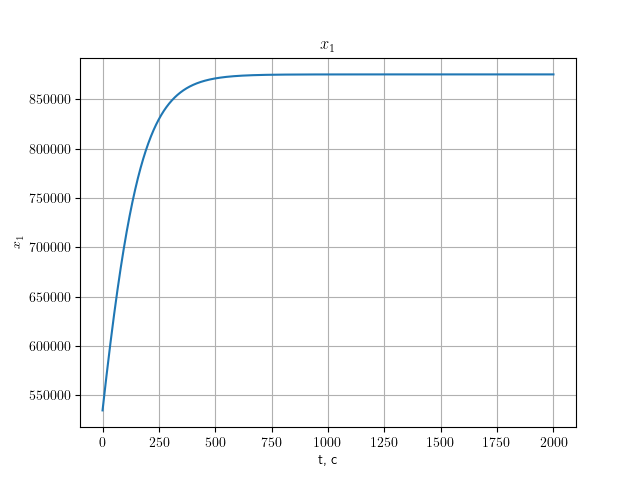
\includegraphics[width=0.32\textwidth]{media/Figure_1.png}} 
			\subfigure[]{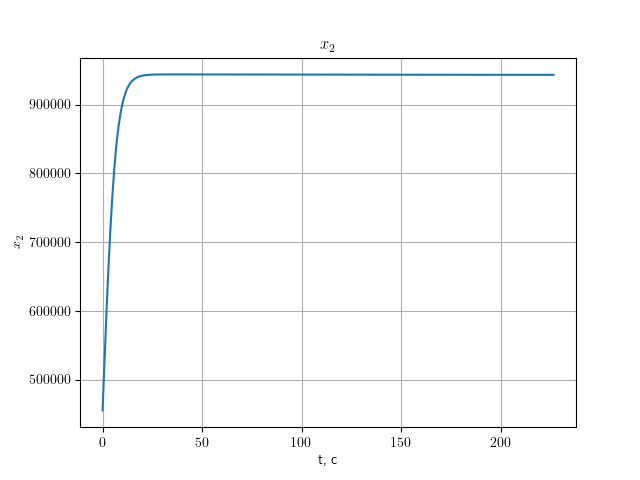
\includegraphics[width=0.32\textwidth]{media/Figure_2.png}}
			\subfigure[]{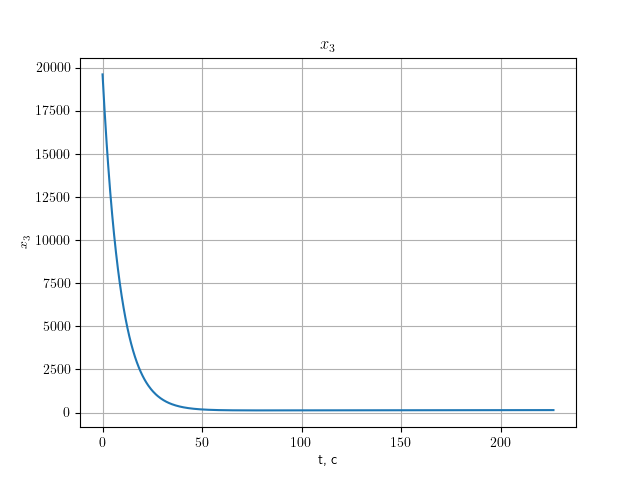
\includegraphics[width=0.32\textwidth]{media/Figure_3.png}}\\
			\subfigure[]{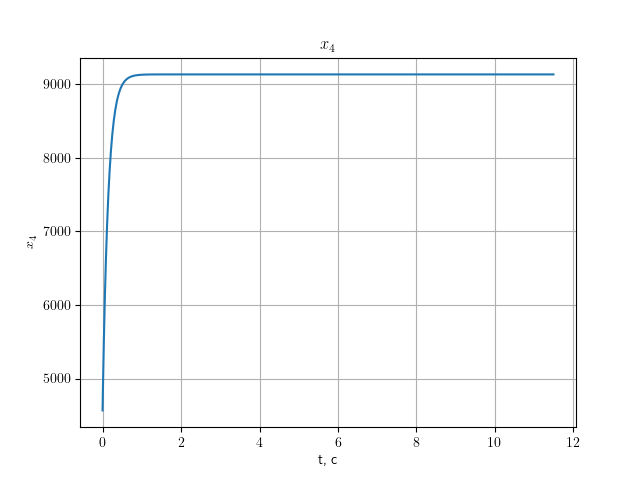
\includegraphics[width=0.40\textwidth]{media/Figure_4.png}}
			\subfigure[]{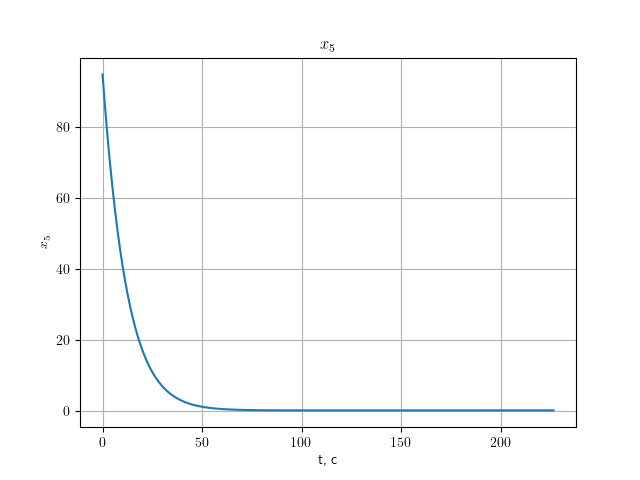
\includegraphics[width=0.40\textwidth]{media/Figure_5.png}}
			\caption{Переходные процессы системы для каждой координаты при выборе начальной точки внутри множества~$D$.}
			\label{fig:in_D}
		\end{figure}
		
		На \figref{fig:in_D} представлены переходные процессы системы при выборе начальной точки внутри множества $D$. Легко заметить, что траектории стремятся к внутреннему положению равновесия $P_3$.
		
		\begin{figure}[h]
			\centering
			\subfigure[]{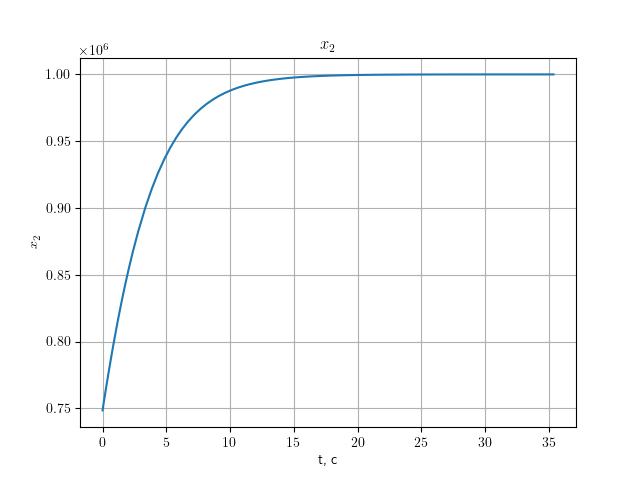
\includegraphics[width=0.40\textwidth]{media/Figure_7.png}} 
			\subfigure[]{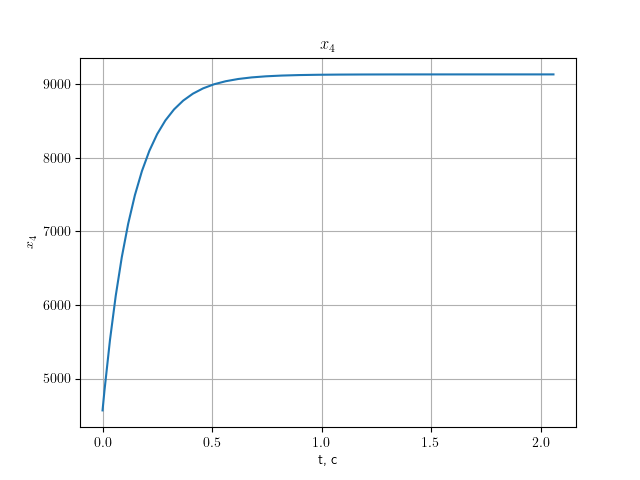
\includegraphics[width=0.40\textwidth]{media/Figure_8.png}}\\
			\caption{Переходные процессы системы координат при выборе начальной точки на на плоскости $x_1=x_3=x_5=0$.}
			\label{fig:on_D_border}
		\end{figure}
		
		Проведем аналогичное моделирование для случайной траектории на плоскости $x_1=x_3=x_5=0$. Из \figref{fig:on_D_border} можно делать вывод о том, что траектория стремится к положению равновесия $P_2$.
		
	\end{example}
	 
	\newpage
	\begin{thebibliography}{1}
		\bibitem{model_params}
		Khajanchi, S., “Uniform Persistence and Global Stability for a Brain Tumor and Immune System Interaction”, \textit{Biophysical Reviews and Letters}, vol. 12, no. 4, pp. 187–208, 2017. doi:10.1142/S1793048017500114.
	\end{thebibliography}
	
\end{document}